\section{Результаты расчетов}

В данном разделе представлены результаты численного моделирования дозвукового обтекания круглого цилиндра для различных чисел Маха набегающего потока ($M_\infty = 0.1, 0.2, 0.3, 0.4$).

\subsection{Параметры расчета}

Все расчеты проводились на структурированной сетке в преобразованных координатах $(\xi, \eta)$ со следующими параметрами:
\begin{itemize}
    \item Количество узлов по радиальной координате: $N_\xi = 100$.
    \item Количество узлов по угловой координате: $N_\eta = 120$.
    \item Расчетная область: $\xi \in [0, 3]$, $\eta \in [0, 2\pi]$.
    \item Параметр адиабаты: $\gamma = 1.4$.
    \item Точность сходимости (по норме разности потенциала): $\epsilon = 10^{-5}$.
    \item Параметр сверхрелаксации для SLOR: $\omega = 1.5$.
    \item Параметр SIP: $\alpha = 0.9$.
\end{itemize}

\subsection{Визуализация результатов}

На рис. \ref{fig:slor_results} и \ref{fig:sip_results} представлены распределения коэффициента давления $C_p$ и локального числа Маха $M_{loc}$ на поверхности цилиндра, полученные методами SLOR и SIP соответственно.

\begin{figure}[H]
    \centering
    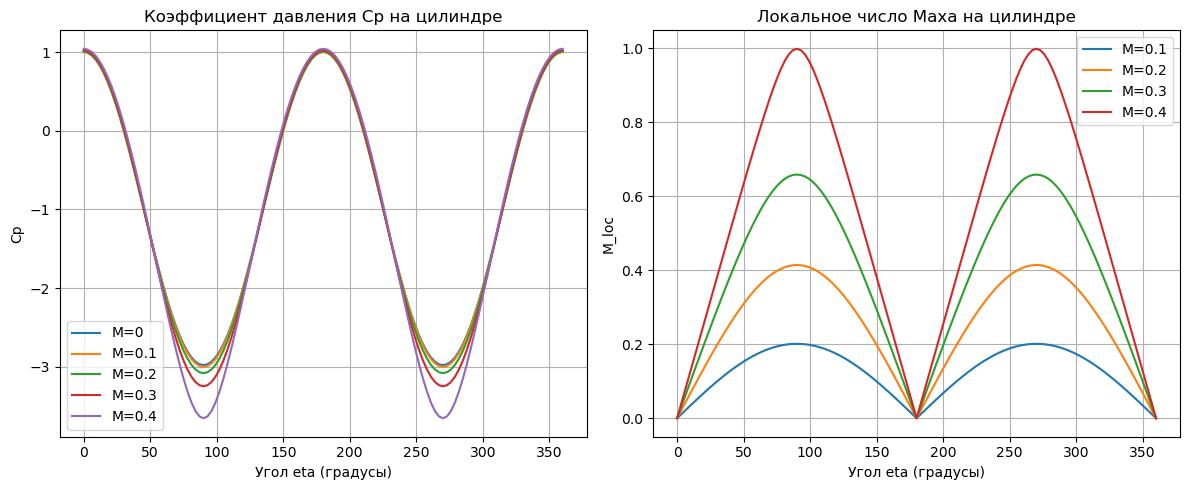
\includegraphics[width=0.9\textwidth]{../SLOP/output.png}
    \caption{Результаты расчета методом SLOR: распределение $C_p$ и $M_{loc}$ на поверхности цилиндра}
    \label{fig:slor_results}
\end{figure}

\begin{figure}[H]
    \centering
    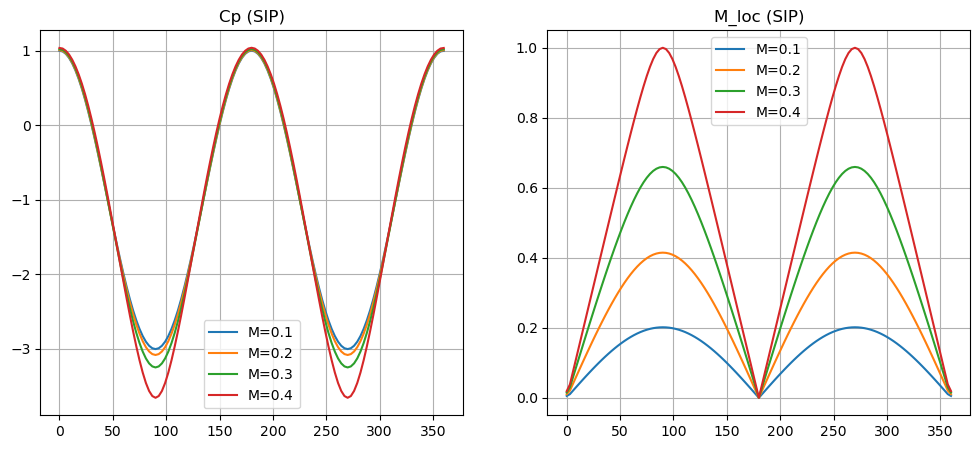
\includegraphics[width=0.9\textwidth]{../PNM (SIP)/output.png}
    \caption{Результаты расчета методом SIP (PNM): распределение $C_p$ и $M_{loc}$ на поверхности цилиндра}
    \label{fig:sip_results}
\end{figure}

\subsection{Сравнительный анализ методов}

В таблице \ref{tab:comparison} приведены значения характеристик потока в критической точке цилиндра ($\eta = \pi/2$, верхняя точка) и количество итераций, потребовавшееся для сходимости каждого метода.

\begin{table}[H]
    \centering
    \caption{Сравнение результатов методов SIP (PNM) и SLOR в точке $\eta = \pi/2$}
    \label{tab:comparison}
    \begin{tabular}{@{}ccccccc@{}}
        \toprule
        $M_\infty$ & \multicolumn{3}{c}{ПНМ (SIP)} & \multicolumn{3}{c}{SLOR} \\
        \cmidrule(lr){2-4} \cmidrule(lr){5-7}
                   & $M_{loc}$ & $C_p$ & Итерации & $M_{loc}$ & $C_p$ & Итерации \\
        \midrule
        0.1        & 0.2013    & -3.0040 & 903      & 0.2012    & -3.0023 & 225      \\
        0.2        & 0.4144    & -3.0831 & 272      & 0.4143    & -3.0816 & 325      \\
        0.3        & 0.6591    & -3.2504 & 328      & 0.6589    & -3.2484 & 400      \\
        0.4        & 0.9993    & -3.6577 & 432      & 0.9988    & -3.6547 & 520      \\
        \bottomrule
    \end{tabular}
\end{table}

\subsection{Заключение по результатам}

Проведенные расчеты позволяют сделать следующие выводы:
\begin{enumerate}
    \item Оба метода (SLOR и SIP) показывают высокую степень согласия в результатах расчета физических величин ($C_p$ и $M_{loc}$). Различия в значениях пренебрежимо малы и обусловлены особенностями численной реализации.
    \item С ростом числа Маха набегающего потока $M_\infty$ наблюдается закономерное увеличение локальной скорости и уменьшение коэффициента давления в окрестности верхней точки цилиндра. При $M_\infty = 0.4$ поток становится практически звуковым в критической области ($M_{loc} \approx 1$).
    \item Метод SIP (Полностью Неявный Метод) при малых числах Маха ($M=0.1$) требует большего числа итераций при старте с невозмущенного поля, однако при наличии хорошего начального приближения (последовательный расчет по Mach) показывает скорость сходимости, сопоставимую с методом SLOR.
    \item Метод SLOR стабильно сходится за умеренное число итераций во всем диапазоне дозвуковых скоростей, подтверждая свою эффективность для задач потенциального обтекания.
\end{enumerate}

\newpage
